\documentclass[a4paper]{article}
\usepackage[utf8]{vietnam}
\usepackage{graphicx}
\usepackage{amssymb}
\usepackage{amsmath}
\usepackage{scrextend}

\usepackage{times}



\title{BIỄU DIỄN TRI THỨC\\ Bài tập 2}
\author{Nhóm 07}
\date{May 29th, 2021}

\begin{document}
	\maketitle
	\begin{center}
		\Large{\textbf{Bài 2 - Bài toán điều chế các chất hóa học}}
	\end{center}
	\section*{Câu a $)$ Tổ chức lưu trữ cho miền tri thức} 
	
	Với phạm vi bài toán, miền tri thức thu thập sẽ nằm trong giới hạn đủ để giải quyết yêu cầu bài toán bao gồm những phương trinh hóa học cần thiết để điều chế \texttt{Na$_2$SO$_4$}, \texttt{H$_2$SO$_4$}, \texttt{HCl} và \texttt{Na} từ \texttt{S}, \texttt{H$_2$O},và \texttt{NaCl} như:\\
	
	
	\texttt{NaCl} = \texttt{Na} = \texttt{Cl$_2$}  
	
	
	\texttt{Na} + \texttt{H$_2$SO$_4$} = \texttt{Na$_2$SO$_4$} + \texttt{SO$_2$} + \texttt{H$_2$O}\\
	
	Sau khi được thu thập, những tri thức này cần được lưu trữ trong tập tin văn bản có cấu trúc \textbf{txt} gồm những quy ước về nguyên tố, hợp chất hóa học, cũng như mối quan hệ giữa chất điều chế và chất được điều chế giúp máy tính hiểu và tính toán được.
		
	\begin{figure}[h]
	\centering
	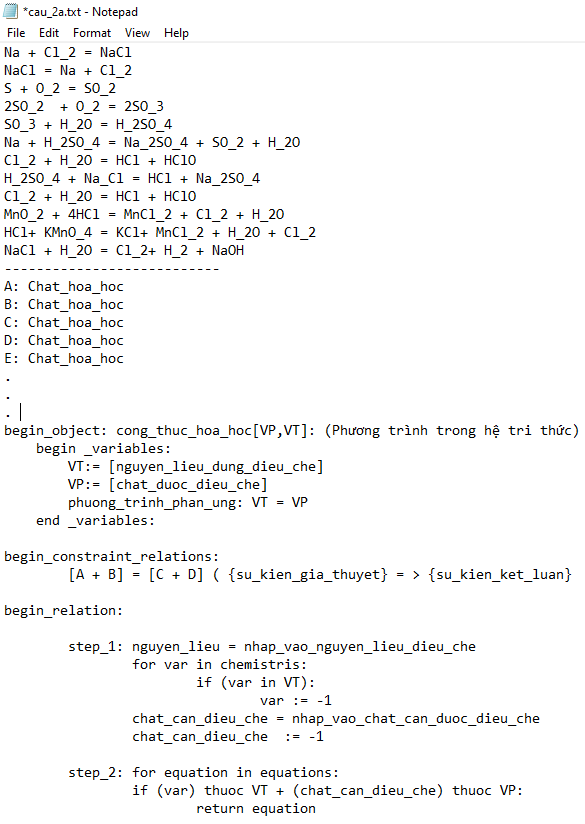
\includegraphics[width=.46\linewidth]{2a_luutru.PNG}  
	\caption{Tổ chức lưu trữ cho miền tri thức điều chế hóa chất}
	\label{}
	\end{figure}


	\section*{Câu b}
	Trình bày thuật giải
	
	\section*{Câu c}
	Cài đặt chương trình

\end{document}